\documentclass{article}
\usepackage{amsmath} % For align*
\usepackage{graphicx} % For images
\usepackage{siunitx} % For units
\graphicspath{{./images/}}

\title{Advanced Engineering Mathematics Partial Differential Equations by Dennis G. Zill Notes}
\author{Chris Doble}
\date{November 2023}

\DeclareMathOperator{\erf}{erf}
\DeclareMathOperator{\erfc}{erfc}

\begin{document}

\maketitle

\tableofcontents

\setcounter{section}{11}
\section{Orthogonal Functions and Fourier Series}

\subsection{Orthogonal Functions}

\begin{itemize}
  \item The \textbf{inner product} of two functions $f_1$ and $f_2$ on an interval $[a, b]$ is the number \[(f_1, f_2) = \int_a^b f_1(x) f_2(x) \,d x.\]

  \item Two functions $f_1$ and $f_2$ are said to be orthogonal on an interval if $(f_1, f_2) = 0$.

  \item A set of real-valued functions $\{\phi_1(x), \phi_2(x), \ldots, \phi_n(x)\}$ is said to be \textbf{orthogonal} on an interval if \[(\phi_i, \phi_j) = 0 \text{ for } i \ne j.\]

  \item The \textbf{square norm} of a function is \[||\phi_n(x)||^2 = (\phi_n, \phi_n)\] and thus its \textbf{norm} is \[||\phi_n(x)|| = \sqrt{(\phi_n, \phi_n)}.\]

  \item An \textbf{orthonormal set} of functions is an orthogonal set of functions that all have a norm of $1$.

  \item An orthogonal set can be made into an orthonormal set by dividing each member by its norm.

  \item If $\{\phi_n(x)\}$ is an infinite orthogonal set of functions on an interval $[a, b]$ and $f(x)$ is an arbitrary function, then it's possible to determine a set of coefficients $c_n, n = 0, 1, 2, \ldots$ such that \[f(x) = \sum_{n = 0}^\infty c_n \phi_n(x) = c_0 \phi_0(x) + c_1 \phi_1(x) + \ldots + c_n \phi_n(x) + \ldots\] This is called an \textbf{orthogonal series expansion} of $f$ or a \textbf{generalized Fourier series} where the coefficients are given by \[c_n = \frac{(f, \phi_n)}{||\phi_n||^2}.\]

  \item A set of real-valued functions $\{\phi_n(x)\}$ is said to be \textbf{orthogonal with respect to a weight function} $w(x)$ on the interval $[a, b]$ if \[\int_a^b w(x) \phi_m(x) \phi_n(x) \,d x = 0,\ m \ne n.\]
\end{itemize}

\subsection{Fourier Series}

\begin{itemize}
  \item The \textbf{Fourier series} of a function $f$ defined on the interval $(-p, p)$ is given by \[f(x) = \frac{a_0}{2} + \sum_{n = 1}^\infty \left( a_n \cos \frac{n \pi}{p} x + b_n \sin \frac{n \pi}{p} x \right)\] where \begin{align*}
          a_0 & = \frac{1}{p} \int_{-p}^p f(x) \,d x                        \\
          a_n & = \frac{1}{p} \int_{-p}^p f(x) \cos \frac{n \pi}{p} x \,d x \\
          b_n & = \frac{1}{p} \int_{-p}^p f(x) \sin \frac{n \pi}{p} x \,d x
        \end{align*}

  \item At points of discontinuity in $f$, the Fourier series takes on the average of the values either side of it.

  \item The Fourier series of a function $f$ gives a \textbf{periodic extension} of the function outside the interval $(-p, p)$.
\end{itemize}

\subsection{Fourier Cosine and Sine Series}

\begin{itemize}
  \item A function $f$ is said to be \textbf{even} if \[f(-x) = f(x)\] and \textbf{odd} if \[f(-x) = -f(x).\]

  \item Even and odd functions have some interesting properties:

        \begin{itemize}
          \item The product of two even functions is even.

          \item The product of two odd functions is even.

          \item The product of an even function and an odd function is odd.

          \item If $f$ is even, then $\int_{-a}^a f(x) \,d x = 2 \int_0^a f(x) \,d x$.

          \item If $f$ is odd, then $\int_{-a}^a f(x) \,d x = 0$.
        \end{itemize}

  \item In light of this, if a function $f$ is even its Fourier coefficients are \begin{align*}
          a_0 & = \frac{2}{p} \int_0^p f(x) \,d x                        \\
          a_n & = \frac{2}{p} \int_0^p f(x) \cos \frac{n \pi}{p} x \,d x \\
          b_n & = 0.
        \end{align*} The series consists of cosine terms and is called the \textbf{Fourier cosine series}.

  \item Similarly, if $f$ is odd then \begin{align*}
          a_n & = 0,\ n = 0, 1, 2, \ldots                                 \\
          b_n & = \frac{2}{p} \int_0^p f(x) \sin \frac{n \pi}{p} x \,d x.
        \end{align*} The series consists of sine terms and is called the \textbf{Fourier sine series}.

  \item Sometimes a Fourier series ``overshoots'' the original value of the function near discontinuities. This is called the \textbf{Gibbs phenomenon}.

  \item Taking the Fourier cosine series of a function $f$ over the interval $[0, L]$ effectively mirrors the function around the vertical axis.

  \item Taking the Fourier sine series of a function $f$ over the interval $[0, L]$ effectively rotates it $\ang{180}$ around the origin.

  \item A particular solution for a nonhomogeneous differential equation with a periodic driving force can be found by taking the Fourier transform of the driving force then using the method of undetermined coefficients to determine the coefficients.
\end{itemize}

\subsection{Complex Fourier Series}

\begin{itemize}
  \item The \textbf{complex Fourier series} of a function $f$ defined on an interval $(-p, p)$ is given by \[f(x) = \sum_{n = -\infty}^\infty c_n e^{i n \pi x / p}\] where \[c_n = \frac{1}{2 p} \int_{-p}^p f(x) e^{-i n \pi x / p} \,d x,\ n = 0, \pm 1, \pm 2, \ldots\]

  \item The \textbf{fundamental period} of a Fourier series is $T = 2 p$.

  \item The \textbf{fundamental angular frequency} of a Fourier series is $\omega = \frac{2 \pi}{T}$.

  \item A \textbf{frequency spectrum} is a plot of the points $(n \omega, |c_n|)$ where $\omega$ is the fundamental angular frequency and $c_n$ are the coefficients of the complex Fourier series. This can be useful to see how each harmonic contributes.
\end{itemize}

\subsection{Sturm-Liouville Problem}

\begin{itemize}
  \item If a boundary value problem contains an arbitrary parameter $\lambda$, the values of $\lambda$ for which the problem has nontrivial solutions are called the \textbf{eigenvalues} of the problem and the associated solutions are called the \textbf{eigenfunctions} of the problem.

  \item An orthogonal set of functions can be generated by solving a two-point boundary-value problem involing a linear second-order differential equation containing a parameter $\lambda$.

  \item A \textbf{regular Sturm-Liouville problem} is a boundary value problem \[\frac{d}{d x} [r(x) y'] + [q(x) + \lambda p(x)] y = 0\] subject to \begin{align*}
          A_1 y(a) + B_1 y'(a) & = 0 \\
          A_2 y(b) + B_2 y'(b) & = 0
        \end{align*} where $p$, $q$, $r$, and $r'$ are real-valued functions continuous on an interval $[a, b]$, $r(x) > 0$ and $p(x) > 0$ for every $x$ in that interval, the coefficients in the boundary conditions are real and independent of $\lambda$, $A_1$ and $B_1$ are not both zero, and $A_2$ and $B_2$ are not both zero.

  \item A boundary condition \[A_1 y(a) + B_1 y'(a) = C\] is said to be \textbf{homogeneous} if $C = 0$ and \textbf{nonhomogeneous} otherwise.

  \item A boundary-value problem consisting of a homogeneous differential equation and a homogeneous boundary condition is said to be homogeneous, otherwise it's nonhomogeneous.

  \item Multiple boundary conditions are said to be \textbf{separated} if each deals with values at a single point $x = a$ and \textbf{mixed} if each deals with values at multiple points $x = a, b, \ldots$

  \item If a boundary-value problem can be identified as a Sturm-Liouville problem we know it has several properties:

        \begin{itemize}
          \item There exists an infinite number of real eigenvalues that can be arranged in increasing order $\lambda_1 < \lambda_2 < \ldots < \lambda_n < \ldots$ such that $\lambda_n \rightarrow \infty$ as $n \rightarrow \infty$.

          \item For each eigenvalue there is only one eigenfunction.

          \item Eigenfunctions corresponding to different eigenvalues are linearly independent.

          \item The set of eigenfunctions corresponding to the set of eigenvalues is orthogonal with respect to the weight function $p(x)$ on the interval $[a, b]$.
        \end{itemize}

  \item If a Sturm-Liouville problem has $r(a) = 0$ and boundary conditions are specified at $x = b$, or $r(b) = 0$ and boundary conditions are specified at $x = a$, then it is called a \textbf{singular boundary-value problem}.

  \item If a Sturm-Liouville problem has $r(a) = r(b)$ and boundary conditions $y(a) = y(b)$, $y'(a) = y'(b)$, then it is called a \textbf{periodic boundary-value problem}.

  \item If the solutions to a singular or periodic boundary-value problem are bounded on the interval $[a, b]$ then the orthogonality relation holds.

  \item Any second-order linear differential equation \[a(x) y'' + b(x) y' + [c(x) + \lambda d(x)] y = 0\] can be transformed into a Sturm-Liouville problem providing the coefficients are continuous and $a(x) \ne 0$ on the interval of interest. This can be done by:

        \begin{enumerate}
          \item dividing by $a$,

          \item multiplying by the integrating factor $e^{\int (b / a) \,d x}$,

          \item recognising that \[e^{\int (b / a) \,d x} y'' + \frac{b}{a} e^{\int (b / a) \,d x} y' = \frac{d}{d x} \left[ e^{\int (b / a) \,d x} y' \right],\]

          \item and rewriting the equation as \[\frac{d}{d x} \left[ e^{\int (b / a) \,d x} y' \right] + \left( \frac{c}{a} e^{\int (b / a) \,d x} + \lambda \frac{d}{a} e^{\int (b / a) \,d x} \right) \lambda = 0\] which is the desired form and lets us recognise \begin{align*}
                  r(x) & = e^{\int (b / a) \,d x}              \\
                  q(x) & = \frac{c}{a} e^{\int (b / a) \,d x}  \\
                  p(x) & = \frac{d}{a} e^{\int (b / a) \,d x}.
                \end{align*}
        \end{enumerate}
\end{itemize}

\subsection{Bessel and Legendre Series}

\subsubsection{Fourier-Bessel Series}

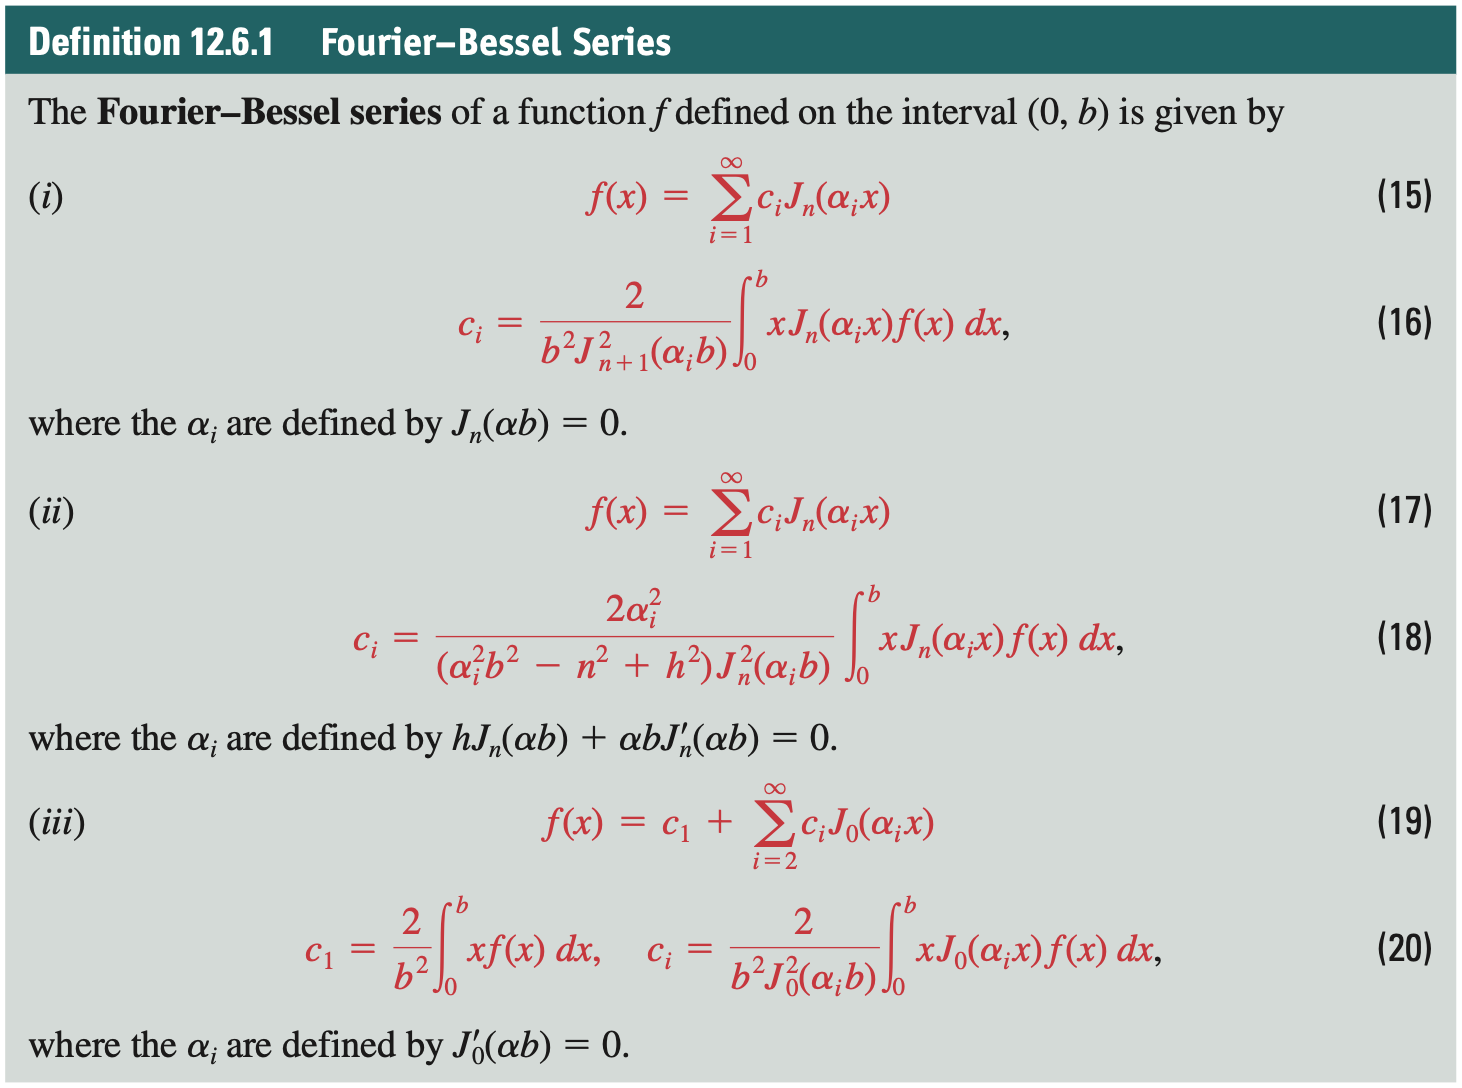
\includegraphics[scale=0.47]{fourier-bessel-series}

\begin{itemize}
  \item The Fourier-Bessel series converges to $f$ where it is continuous and \[\frac{f(x+) + f(x-)}{2}\] where it is discontinuous.
\end{itemize}

\subsubsection{Fourier-Legendre Series}

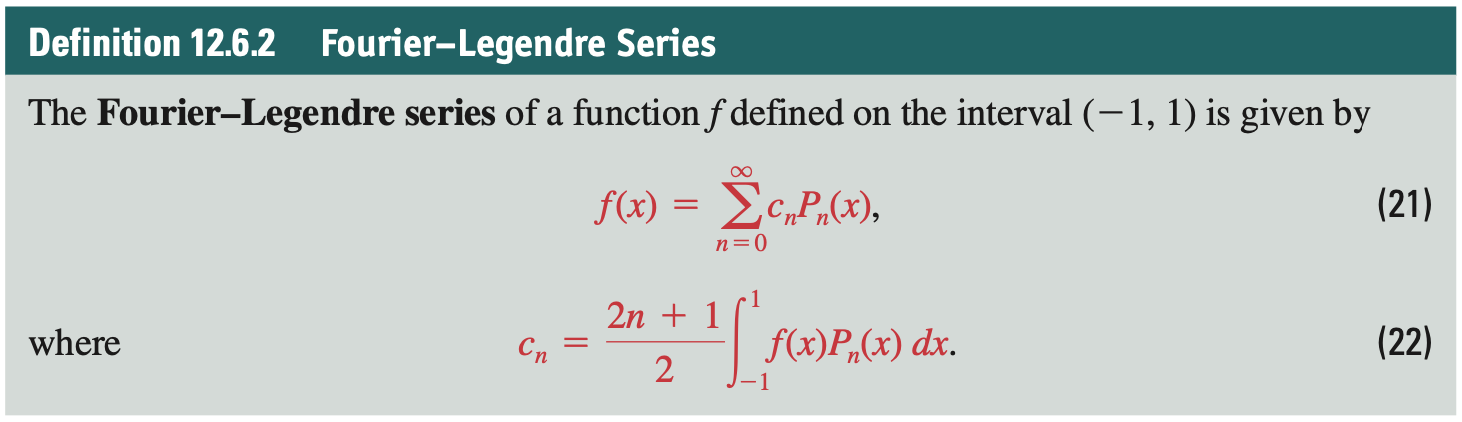
\includegraphics[scale=0.47]{fourier-legendre-series}

\begin{itemize}
  \item The Fourier-Legendre series converges to $f$ where it is continuous and \[\frac{f(x+) + f(x-)}{2}\] where it is discontinuous.
\end{itemize}

\section{Boundary-Value Problems in Rectangular\\Coordinates}

\subsection{Separable Partial Differential Equations}

\begin{itemize}
  \item Like ordinary differential equations (ODEs), partial differential equations (PDEs) can be linear or nonlinear. If the dependent variable and its partial derivatives only appear to the first power, it's a linear PDE.

  \item The general form of a \textbf{linear second-order partial differential equation} is \[A \frac{\partial^2 u}{\partial x^2} + B \frac{\partial^2 u}{\partial x \partial y} + C \frac{\partial^2 u}{\partial y^2} + D \frac{\partial u}{\partial x} + E \frac{\partial u}{\partial y} + F u = G.\] When $G(x, y) = 0$ the equation is said to be \textbf{homogeneous}, otherwise it's \textbf{nonhomogeneous}.

  \item Under the method of \textbf{separation of variables} we assume that the solution of a PDE is a product of functions of each independent variable, e.g. if we seek a solution with independent variables $x$ and $y$ we assume it has the form $u = X(x) Y(y)$. With this assumption it's sometimes possible to reduce the PDE into multiple independent ODEs.

  \item A key step during the process of applying the method of separation of variables is when the equation has been reduced to a form like \[F(X, X', X'') = G(Y, Y', Y'').\] Remembering that $X$ and $Y$ are functions of a single variable, this means that varying $x$ independently of $y$ or vice versa affects one side of the equation but not the other. In order for them to remain equal this means both sides must be constant. This lets us equate each side with a \textbf{separation constant}, giving us an ODE that can be solved on its own.

  \item The \textbf{superposition principle} states that if $u_1, u_2, \ldots, u_n$ are solutions of a homogeneous linear partial differential equation, then the linear combination \[u = c_1 u_1 + c_2 u_2 + \ldots + c_n u_k\] is also a solution.

  \item A linear second-order partial differential equation in two independent variables with constant coefficients \[A \frac{\partial^2 u}{\partial^2 x} + B \frac{\partial^2 u}{\partial x \partial y} + C \frac{\partial^2 y}{\partial y^2} + D \frac{\partial u}{\partial x} + E \frac{\partial u}{\partial y} + F u = G\] can be classified as one of three types:

        \begin{itemize}
          \item \textbf{hyperbolic} if $B^2 - 4 A C > 0$,

          \item \textbf{parabolic} if $B^2 - 4 A C = 0$, and

          \item \textbf{elliptic} if $B^2 - 4 A C < 0$.
        \end{itemize}
\end{itemize}

\subsection{Classical PDEs and Boundary-Value Problems}

\begin{itemize}
  \item The \textbf{one-dimensional heat equation} \[k \frac{\partial^2 u}{\partial x^2} = \frac{\partial u}{\partial t},\ k > 0\] describes the diffusion of thermal energy through a one-dimensional rod where \[k = \frac{K}{\gamma \rho}\] is called the \textbf{thermal diffusivity} of the rod, $K$ is its thermal conductivity, $\gamma$ is its specific heat, and $\rho$ is its density.

  \item The \textbf{one-dimensional wave equation} \[a^2 \frac{\partial^2 u}{\partial x^2} = \frac{\partial^2 u}{\partial t^2}\] describes the motion of a wave through a taut string where \[a^2 = \frac{T}{\rho},\] $T$ is the tension in the string, and $\rho$ is its density per unit length.

  \item If a PDE depends on time $t$, the state of the system at $t = 0$ can be used as \textbf{initial conditions} to help determine the solution.

  \item \textbf{Boundary conditions} state the value of the solution at particular points, e.g. if the ends of a string are fixed in place, and can also help determine the solution.

  \item There are three types of boundary conditions:

        \begin{itemize}
          \item \textbf{Dirichlet conditions} specify the value of $u$ at a particular location, e.g. a particular point on a string is fixed in place.

          \item \textbf{Neumann conditions} specify the value of $\partial u / \partial n$ at a particular location, e.g. a particular point on a string always has $0$ velocity.

          \item \textbf{Robin conditions} specify the value of $\partial u / \partial n + h u$ where $h$ is a constant, e.g. thermal energy is lost at a constant rate at the end of a rod.
        \end{itemize}
\end{itemize}

\subsection{Heat Equation}

\begin{itemize}
  \item Sometimes a solution of a PDE may not satisfy a given boundary condition or initial value. However, if we know that the solution is a member of an infinite orthogonal set of solutions (e.g. via the Sturm-Liouville theorem) then we may be able to use the superposition principle to select constants $c_i$ that do satisfy the boundary condition or initial value.
\end{itemize}

\setcounter{subsection}{4}
\subsection{Laplace's Equation}

\begin{itemize}
  \item A \textbf{Dirichlet problem} is the problem of finding a function which solves a PDE in a particular region given the values the function should take on the boundaries of that region.

  \item The \textbf{maximum principle} states that a solution of Laplace's equation takes on its maximum and minimum values on the boundary of the region in which the solution is defined. Also, the solution can have no relative maxima or minima in the region.

  \item A Dirichlet problem for a rectangle can be solved via separation of variables when homogeneous boundary conditions are specified on two parallel boundaries, but not when the boundary conditions of all four sides are nonhomogeneous. This can be solved by breaking the problem in two: one that has homogeneous boundary conditions on the $x$ axis and another that has them on the $y$ axis. By the superposition principle, adding the solutions to these problems will be a solution to the original problem.
\end{itemize}

\subsection{Nonhomogeneous Boundary-Value Problems}

\begin{itemize}
  \item A BVP involving a time-independent nonhomogeneous equation and time-independent boundary conditions like \begin{align*}
          k \frac{\partial^2 u}{\partial x^2} + F(x) & = \frac{\partial u}{\partial t} \\
          u(0, t)                                    & = u_0                           \\
          u(L, t)                                    & = u_1                           \\
          u(x, 0)                                    & = f(x)
        \end{align*} can be solved by substituting \[u(x, t) = v(x, t) + \psi(x).\] This decomposes the problem into two: an ODE in $\psi(x)$ with nonhomogeneous boundary conditions \begin{align*}
          k \psi'' + F(x) & = 0    \\
          \psi(0)         & = u_1  \\
          \psi(1)         & = u_2,
        \end{align*} and a PDE in $v(x, t)$ with homogeneous boundary conditions \begin{align*}
          k \frac{\partial^2 v}{\partial x^2} & = \frac{\partial v}{\partial t} \\
          v(0, t)                             & = 0                             \\
          v(L, t)                             & = 0                             \\
          v(x, 0)                             & = f(x) - \psi(x).
        \end{align*} We can then solve the ODE for $\psi(x)$, substitute the result into the PDE, and solve for $v(x, t)$, giving us $u(x, t)$.

  \item A BVP involving a time-dependent nonhomogeneous equation and time-dependeny boundary conditions like \begin{align*}
          k \frac{\partial^2 u}{\partial x^2} + F(x, t) & = \frac{\partial u}{\partial t} \\
          u(0, t)                                       & = u_0(t)                        \\
          u(L, t)                                       & = u_1(t)                        \\
          u(x, 0)                                       & = f(x)
        \end{align*} can be solved via the following steps:

        \begin{enumerate}
          \item Substitute \begin{align*}
                  u(x, t) & = v(x, t) + \psi(x, t)                             \\
                          & = v(x, t) + u_0(t) + \frac{x}{L} [u_1(t) - u_0(t)]
                \end{align*} which changes the BVP to \begin{align*}
                  k \frac{\partial^2 v}{\partial x^2} + G(x, t) & = \frac{\partial v}{\partial t} \\
                  v(0, t)                                       & = 0                             \\
                  v(L, t)                                       & = 0                             \\
                  v(x, 0)                                       & = f(x) - \psi(x, 0)
                \end{align*} where $G(x, t) = F(x, t) - \frac{\partial \psi}{\partial t}$.

          \item Assuming $G(x, t)$ can be expressed as a Fourier sine series, find the coefficients of that series $G_n(t)$.

          \item Assuming $v(x, t)$ can also be expressed as a Fourier sine series, express the BVP in $v(x, t)$ using such a series and the series for $G(x, t)$.

          \item Equate the coefficients of the two series to get an ODE for the $v(x, t)$ series coefficients $v_n(t)$.

          \item Solve the ODE to find $v_n(t)$ and thus express $v(x, t)$ as a Fourier sine series with coefficients $C_n$.

          \item Use the boundary conditions of the BVP in $v(x, t)$ to solve for $C_n$.

          \item Subsitute $C_n$ to find $v(x, t)$.

          \item Substitute $v(x, t)$ to find $u(x, t)$.
        \end{enumerate}

  \item If a BVP includes a time-dependent term $F(x, t)$ in the PDE but has homogeneous boundary conditions, $\psi(x, t)$ will be $0$ and there's no need to substitute $u(x, t) = v(x, t) + \psi(x, t)$. The BVP can be solved by proceeding from step 2 above, replacing $G(x, t)$ with $F(x, t)$ and $v(x, t)$ with $u(x, t)$.
\end{itemize}

\subsection{Orthogonal Series Expansion}

\begin{itemize}
  \item For certain types of boundary conditions, the method of separation of variables and the superposition principle can lead to infinite series that aren't Fourier series. If a series is a result of a Sturm-Liouville problem its eigenfunctions $\phi_n$ are orthogonal and can still be used to solve the BVP, but the coefficients must be calculated using the general formula \[A_n = \frac{(f, \phi_n)}{||\phi_n||^2}.\]
\end{itemize}

\subsection{Fourier Series in Two Variables}

\begin{itemize}
  \item Two-dimensional BVPs can also be solved via separation of variables. The process is similar, however when separating the variables you'll get something like \[\frac{X''}{X} = -\frac{Y''}{Y} + \frac{T'}{k T}.\] Introduction a constant leads to \begin{align*}
          \frac{X''}{X}                   & = -\lambda \\
          -\frac{Y''}{Y} + \frac{T'}{k T} & = -\lambda
        \end{align*} and introduction of another constant leads to \begin{align*}
          \frac{Y''}{Y}            & = -\mu  \\
          \frac{T'}{k T} + \lambda & = -\mu.
        \end{align*} These three BVPs can then be solved independently with the final resulting including a double sum over two infinite series.

  \item If the result includes an infinite sine series (a \textbf{sine series in two variables} or a \textbf{double sine series}) the coefficients are \[A_{m n} = \frac{4}{b c} \int_0^c \int_0^b f(x, y) \sin \frac{m \pi}{b} x \sin \frac{n \pi}{c} y \,d x \,d y\] where $b$ is the width of the region and $c$ is its height.

  \item If the result includes an infinite cosine series (a \textbf{cosine series in two variables} or a \textbf{double cosine series}) the coefficients are more complicated as there is an zero constant in each dimension, resulting in four equations for $A_{0 0}$, $A_{m 0}$, $A_{0 n}$, and $A_{m n}$.
\end{itemize}

\section{Boundary-Value Problems in Other Coordinate Systems}

\subsection{Polar Coordinates}

\begin{itemize}
  \item The Laplacian of a function $u(r, \theta)$ in polar coordinates is \[\nabla^2 u = \frac{\partial^2 u}{\partial r^2} + \frac{1}{r} \frac{\partial u}{\partial r} + \frac{1}{r^2} \frac{\partial^2 u}{\partial \theta^2}.\]

  \item Thus, the Laplace equation in polar coordinates corresponds to two boundary value problems \begin{align*}
          r^2 R'' + r R' - \lambda R & = 0  \\
          \Theta'' + \lambda \Theta  & = 0.
        \end{align*}

  \item Some implicit constraints on a boundary value problem in polar coordinates are: $R(r)$ must be bounded at $r = 0$, and $\Theta(\theta)$ must be $2 \pi$ periodic (assuming the problem concerns a full circle).
\end{itemize}

\subsection{Cylindrical Coordinates}

\begin{itemize}
  \item The two-dimensional heat and wave equations in polar coordinates are \begin{align*}
          k \left( \frac{\partial^2 u}{\partial r^2} + \frac{1}{r} \frac{\partial u}{\partial r} + \frac{1}{r^2} \frac{\partial^2 u}{\partial \theta^2} \right)   & = \frac{\partial u}{\partial t} \text{, and} \\
          a^2 \left( \frac{\partial^2 u}{\partial r^2} + \frac{1}{r} \frac{\partial u}{\partial r} + \frac{1}{r^2} \frac{\partial^2 u}{\partial \theta^2} \right) & = \frac{\partial^2 u}{\partial t^2}.
        \end{align*} For problems with radial symmetry they reduce to \begin{align*}
          k \left( \frac{\partial^2 u}{\partial r^2} + \frac{1}{r} \frac{\partial u}{\partial r} \right)   & = \frac{\partial u}{\partial t} \text{, and} \\
          a^2 \left( \frac{\partial^2 u}{\partial r^2} + \frac{1}{r} \frac{\partial u}{\partial r} \right) & = \frac{\partial^2 u}{\partial t^2}.
        \end{align*}

  \item Differential equations of the form \[x^2 y'' + x y' + (\alpha^2 x^2 - p^2) y = 0,\ \alpha > 0\] are parametric Bessel equations of order $p$ and have solutions \[c_1 J_p(\alpha x) + c_2 Y_p(\alpha x)\] where $J_p$ and $Y_p$ are Bessel functions of the first- and second-kind, respectively.

  \item The Laplacian in cylindrical coordinates is \[\nabla^2 u = \frac{\partial^2 u}{\partial r^2} + \frac{1}{r} \frac{\partial u}{\partial r} + \frac{1}{r^2} \frac{\partial^2 u}{\partial \theta^2} + \frac{\partial^2 u}{\partial z^2}.\]
\end{itemize}

\section{Integral Transform Method}

\subsection{Error Function}

\begin{itemize}
  \item The \textbf{error function} $\erf(x)$ and the \textbf{complementary error function} $\erfc(x)$ are defined as \begin{align*}
          \erf(x)  & = \frac{2}{\sqrt{\pi}} \int_0^x e^{-u^2} \,du \text{, and} \\
          \erfc(x) & = \frac{2}{\sqrt{\pi}} \int_x^\infty e^{-u^2} \,d u.
        \end{align*}

  \item The error function can be thought of as the area under the graph of $f(t) = (2 / \sqrt{\pi}) e^{-t^2}$ on the interval $[0, x]$ and the complementary error function can be thought of the area under the same graph on the interval $[x, \infty)$.

  \item Some properties of $\erf$ and $\erfc$ include:

        \begin{itemize}
          \item their domains are $(-\infty, \infty)$,

          \item they are continuous,

          \item $\erf(x)$ is an odd function,

          \item $\erf(0) = 0$,

          \item $\erfc(0) = 1$,

          \item $\lim_{x \rightarrow \infty} \erf(x) = 1$,

          \item $\lim_{x \rightarrow \infty} \erfc(x) = 0$,

          \item $\lim_{x \rightarrow -\infty} \erf(x) = -1$, and

          \item $\lim_{x \rightarrow -\infty} \erfc(x) = 2$.
        \end{itemize}
\end{itemize}

\subsection{Applications of the Laplace Transform}

\begin{itemize}
  \item Applying the Laplace transform to a PDE turns it into an ODE.

  \item The Laplace transform of $u(x, t)$ with respect to $t$ is \[\mathcal{L}\{u(x, t)\} = \int_0^\infty e^{-s t} u(x, t) \,d t = U(x, s).\]

  \item The properties of the Laplace transform when applied to single-valued functions also apply to multi-valued functions, e.g. \begin{align*}
          \mathcal{L} \left\{ \frac{\partial u}{\partial t} \right\}     & = s U(x, s) - u(x, 0)                  \\
          \mathcal{L} \left\{ \frac{\partial^2 u}{\partial t^2} \right\} & = s^2 U(s, x) - s u(x, 0) - u_t(x, 0).
        \end{align*}

  \item Since we are transforming with respect to $t$, it's valid that differentiation with respect to $x$ be ``pulled out the front'' \[\mathcal{L} \left\{ \frac{d^2 u}{d x^2} \right\} = \frac{d^2}{d x^2} \mathcal{L}\{u(x, t)\}.\]

  \item The general procedure to solve a PDE BVP using the Laplace transform is:

        \begin{enumerate}
          \item Apply the Laplace transform to both sides of the equation and the boundary conditions.

          \item Solve the resulting ODE for $U(x, s)$.

          \item Apply the inverse laplace transform to $U(x, s)$ to find $u(x, t)$.
        \end{enumerate}
\end{itemize}

\subsection{Fourier Integral}

\begin{itemize}
  \item The Fourier series can only be used to represent functions that are periodic on an interval $[-p, p]$ or $[0, L]$. The \textbf{Fourier integral} can be used to represent some nonperiodic functions on the interval $(-\infty, \infty)$.

  \item The Fourier integral of a function $f$ defined on an interval $(-\infty, \infty)$ is given by \[f(x) = \frac{1}{\pi} \int_0^\infty [A(\alpha) \cos \alpha x + B(\alpha) \sin \alpha x] \,d \alpha\] where \begin{align*}
          A(\alpha) & = \int_{-\infty}^\infty f(x) \cos \alpha x \,d x \text{, and} \\
          B(\alpha) & = \int_{-\infty}^\infty f(x) \sin \alpha x \,d x.
        \end{align*}

  \item The Fourier integal of an even function on the interval $(-\infty, \infty)$ is the \textbf{cosine integral} \[f(x) = \frac{2}{\pi} \int_0^\infty A(\alpha) \cos \alpha x \,d \alpha\] where \[A(\alpha) = \int_0^\infty f(x) \cos \alpha x \,d x.\]

  \item Taking the cosine integral of a function that isn't even effectively mirrors it around the $y$-axis.

  \item The Fourier integal of an odd function on the interval $(-\infty, \infty)$ is the \textbf{sine integral} \[f(x) = \frac{2}{\pi} \int_0^\infty A(\alpha) \sin \alpha x \,d \alpha\] where \[A(\alpha) = \int_0^\infty f(x) \sin \alpha x \,d x.\]

  \item Taking the sine integral of a function that isn't odd effectively mirrors it around the origin.

  \item The Fourier integral can also be expressed in complex form \[f(x) = \frac{1}{2 \pi} \int_{-\infty}^\infty C(\alpha) e^{-i \alpha x} \,d \alpha\] where \[C(\alpha) = \int_{-\infty}^\infty f(x) e^{i \alpha x} \,d x.\]
\end{itemize}

\end{document}